\chapter{Explication of the problem}

\medskip
\textbf{During this project, we will only study cylinder object.}
A lot of information given here come from this document \cite{EDP}

\section{Explication of the context}

Let consider here a cylinder object which is excited by a plane wave. This problem is independent of the z-dimension so we can consider a two dimension problem.
We will need to switch between a Cartesian landmark and a polar landmark.
\begin{figure}[H]
\centering
    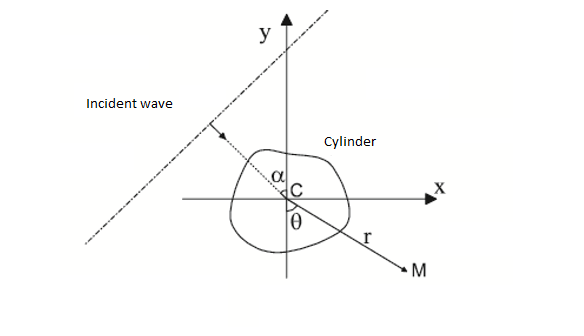
\includegraphics[scale=1,angle=0]{Image2.png}
    \caption{General situation of the problem.}
    \label{fig:Image2}
\end{figure}

Here, $\alpha$ is the incident angle of the wave and $r and \theta$ are the polar position of the point $M$. Furthermore, the center of the cylinder is at the same place of the origin. 

\section{Equations}


The wave equation can be written as follows:

\begin{equation}
 (\nabla + k^2).p = 0 
\end{equation}

In cylinder landmark, this result become :

\begin{equation}
 \frac{1}{r}\frac{\partial}{\partial r}(
 \frac{ r \partial p}{\partial r}) + \frac{1}{r^2}\frac{\partial^2 p}{\partial \theta^2} + \frac{\partial^2 p}{\partial z^2} + k^2 p = 0 
\end{equation}

The problem is independent of the z-dimension so we obtain :

\begin{equation}
 \frac{1}{r}\frac{\partial}{\partial r}(
 \frac{ r \partial p}{\partial r}) + \frac{1}{r^2}\frac{\partial^2 p}{\partial \theta^2} + k^2 p = 0 
\end{equation}

This problem allows us to use the separation of variables (also known as the Fourier method) and allows to rewrite an equation so that each of two variables occurs on a different side of the equation. The set of solution p can be write as:

\begin{equation}
 p(r,\theta) = R(r).\Theta(\theta)
\end{equation}

Thanks to the separation of variable, we know that we have a family of solution which is countable so we can write:

\begin{equation}
p_{n}(r,\theta) = R_{n}(r).\Theta_{n}(\theta)
\end{equation}

The function $\Theta$ is $2\pi$ periodic so it can be write as:

\begin{equation}
\Theta_{n}(\theta) = a_{n}.e^{in\theta} + b_{n}.e^{-in\theta}
\end{equation}

Thanks to the Bessel and Hankel functions, we can express the solution:

\begin{equation}
R_{n} = c_{n}.J_{n}(kr) + d_{n}.Y_{n}(kr)
\end{equation}

Or:

\begin{equation}
R_{n} = c_{n}.H^{(1)}_{n}(kr) + d_{n}.H^{(2)}_{n}(kr)
\end{equation}

The set of solution can be express by the functions:

\begin{equation}
J_{n}(kr)e^{in\theta} \qquad Y_{n}(kr)e^{-in\theta}  \qquad    n\in \mathbb{Z}
\end{equation}

\begin{equation}
H^{(1)}_{n}(kr)e^{in\theta} \qquad H^{(2)}_{n}(kr)e^{-in\theta}  \qquad    n\in \mathbb{Z}
\end{equation}

We will have two waves:
\begin{itemize}
\item An incident wave $p_{inc}$.
\item A diffused wave $p_{dif}$ resulted from the reaction of the incident wave and the object.
\end{itemize}

\chapter{Expression of the wave resulting of this situation.}

Both the incident wave and the diffused wave have to be defined at (0,0) and mustn't diverge for $r\rightarrow +\infty$.

The consequences are that the incident wave can be written as :

\begin{equation}
p_{inc} =  	\sum_{n=-\infty}^{\infty} a_n J_{n}(kr)e^{in\theta} 
\end{equation}

If we choose to use the Hankel functions in order to express the diffused wave, we get the result:

\begin{equation}
p_{dif} =  	\sum_{n=-\infty}^{\infty} b_{n}H^{(1)}_{n}(kr)e^{in\theta}
\end{equation}

The limit condition which applies here is the SOMMERFELD condition. That means that:

\begin{equation}
p_{inc}(r,\theta) = p_{dif}(r,\theta) \qquad \forall(r,\theta) \in \{Border\, of\, the\, object\}
\end{equation}

Thanks to the fact each terms are independent, we have:

\begin{equation}
b_{n}.H^{(1)}_{n}(kr) = a_n J_{n}(kr) \qquad \forall n \in \mathbb{N} \qquad \forall(r,\theta) \in \{Border\, of\, the\, object\}
\end{equation}

So we have a relation between the coefficient $a_n$ and $b_n$. We still have to find an expression for $a_n$.

The wave $p_{inc}$ is a plane wave which means that it can be write as:

\begin{equation}
p_{inc} = e^{i k_{inc} x} \qquad or \qquad p_{inc} = e^{i k_{inc} r.\cos( \theta - \alpha )}
\end{equation}

If we develop the term $\cos(\theta-\alpha)$ as a Fourier series, we get the equation:

\begin{equation}
p_{inc} =  	\sum_{n=-\infty}^{\infty} i^n e^{-i n \alpha} J_{n}(kr)e^{in\theta} 
\end{equation}

Which means $a_n = i^n e^{-i n \alpha} $. With this, we can express the wave resulting to the diffraction of the incident wave on the object.

\chapter{Examples of situation encountered.}

During this project, we will have only two situation.

We will in a first step consider a unique  cylinder which its radius change through time and we will study the magnetic field at the point M:

\begin{figure}[H]
\centering
    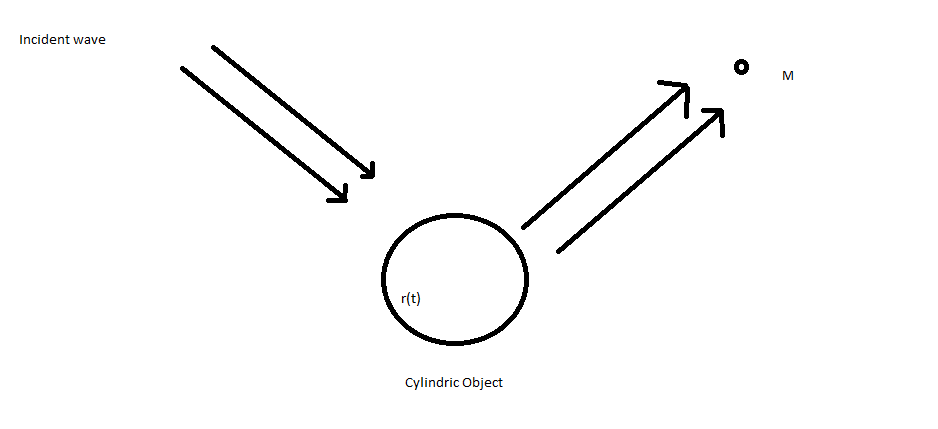
\includegraphics[scale=0.6,angle=0]{Image3.png}
    \caption{Study with a unique object.}
    \label{fig:Image3}
\end{figure}

In a second step, we will consider a lot of cylinders which can move through time and study the magnetic field at the point M: 

\begin{figure}[H]
\centering
    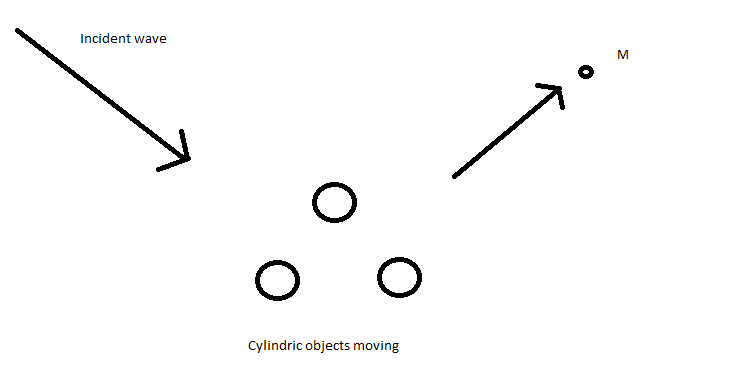
\includegraphics[scale=0.6,angle=0]{Image4.png}
    \caption{Study with a set of object.}
    \label{fig:Image4}
\end{figure}

For this situation, we have to estimate the phase shift between those objects and an origin. Thanks to some geometric theorems, this can be easily obtain. 


\bigskip

\paragraph{Conclusion}
The code needed in order to generate those signals is already working and all we need is to simulate the movement and the deformation of one or two cylinders and see the effect of the movement and the form deformation on the electromagnetic signature.

%\begin{figure}[H]
%\centering
%    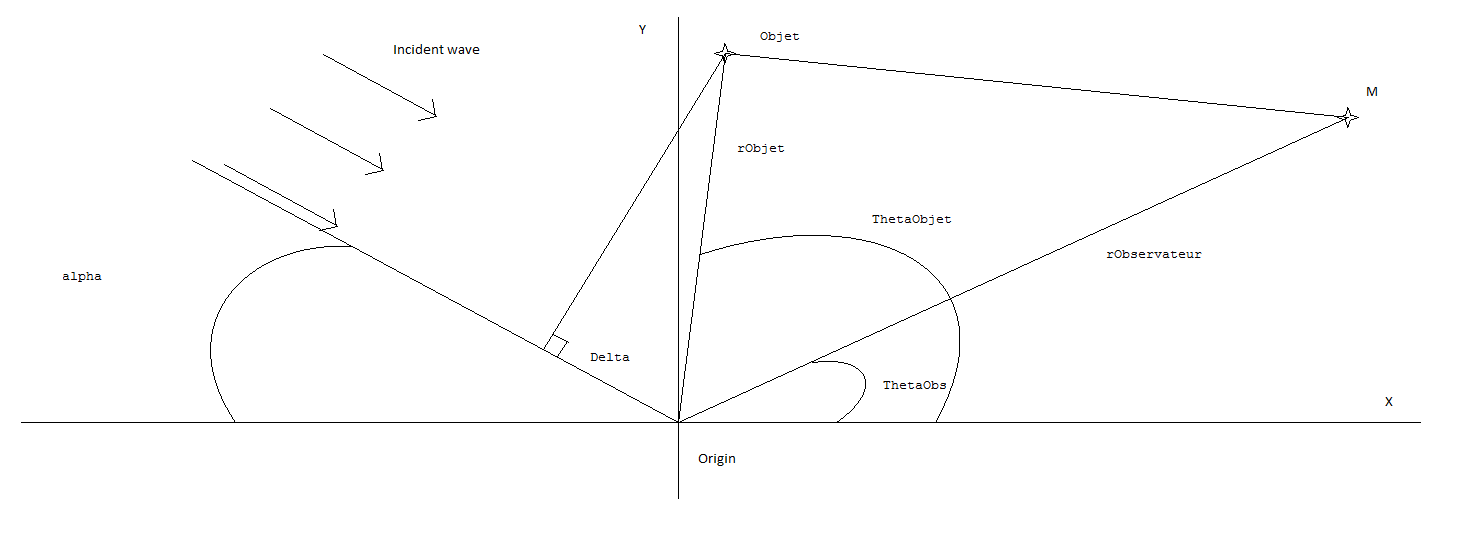
\includegraphics[scale=0.4,angle=90]{diffrac.png}
%    \caption{phase-shift between an object and the origin.}
%    \label{fig:diffrac}
%\end{figure}